\chapter{\"Ubersicht} 

Ein Test gilt als erfolgreich bestanden, wenn er alle \"Uberpr\"ufungen besteht, keine ungewollten Fehlermeldungen wirft und nicht vorzeitig abbricht.
\newline
Zudem erf\"ullen alle Unittests, die erfolgreich bestanden sind, die Bedingungen aller in den Sektionen gennanten Test-Frameworks f\"ur erfolgreiches Bestehen.

\begin{table}[H]
\centering
\renewcommand\arraystretch{1.5}
\begin{tabular}{|L{10cm}|c| }
\hline
Der Test wurde erfolgreich bestanden & \testGood \\ \hline
Der Test wurde erfolgreich bestanden, allerdings nur unter der Vorraussetzung, dass ben\"otigte andere Komponenten (z.B. Graphite, Datenbank) erreichbar sind & \testOk \\ \hline
Der Test ist fehlgeschlagen & \testBad \\ \hline
\end{tabular}
\end{table}

\newpage
\renewcommand\arraystretch{1.1}
\section{Unittests}

F\"ur die Code-\"Uberdeckung der folgenden Tests wurden JUnit 4.8.2 und kafka-streams-test-utils 1.1.0 verwendet.
\newline
Die verwendete Kafka-Version weicht minimal von der vorgegeben Testumgebung ab, da f\"ur die f\"ur uns vorgegebene Version keine kafka-streams-test-utils version existierte. Es wird Kafka 1.0.1 mit der Testumgebung f\"ur 1.1.0 verwendet.
\subsection{ObservationDataDeserializer}
\begin{table}[H]
\centering
\begin{tabular}{|L{9cm}|c| }
\hline
Funktion & \\
\hline
serialisiertes Objekt deserialisieren & \testGood \\
\hline
\end{tabular}
\end{table}

\subsection{GeoRectangle}
\begin{table}[H]
\centering
\begin{tabular}{|L{9cm}|c| }
\hline
Funktion & \\
\hline
anzahl an Sensoren (mit Einschr\"ankung) auslesen & \testGood \\ \hline
gemittelte Sensordaten auslesen & \testGood \\ \hline
Sub-Polygon-Cluster generieren & \testGood \\ \hline
GeoJson des Polygons generieren (mit Wert zu einer Eigenschaft) & \testGood \\ \hline
pr\"ufen ob ein Punkt enthalten ist & \testGood \\ \hline
alle SensorIDs zur\"uckgeben lassen und \"uberpr\"ufen & \testGood \\ \hline
\end{tabular}
\end{table}

\subsection{GeoRecRectangleGrid}
\begin{table}[H]
\centering
\begin{tabular}{|L{9cm}|c| }
\hline
Funktion & \\
\hline
einen Sensor zum Grid hinzuf\"ugen & \testGood \\ \hline
die enthaltenen Eigenschaften (z.B. temperature\textunderscore celsius) \"uberpr\"ufen & \testGood \\ \hline
Daten des kompletten Grids an Graphite senden & \testOk \\ \hline
zwei Grids auf Equivalenz testen & \testGood \\ \hline
\end{tabular}
\end{table}

\subsection{GridPropertiesFileManager}
\begin{table}[H]
\centering
\begin{tabular}{|L{9cm}|c| }
\hline
Funktion & \\ \hline
initialisierendes laden der Eigenschaften & \testGood \\ \hline
\end{tabular}
\end{table}

\subsection{GradientPropertiesFileManager}
\begin{table}[H]
\centering
\begin{tabular}{|L{9cm}|c|}
\hline
Funktion & \\
\hline
initialisierendes laden der Eigenschaften & \testGood \\ \hline
\end{tabular}
\end{table}

\subsection{KafkaPropertiesFileManager}
laden und \"uberpr\"ufen der..
\begin{table}[H]
\centering
\begin{tabular}{|L{9cm}|c|}
\hline
Funktion & \\
\hline
Dummy-Stream Eigenschaften & \testGood \\ \hline
Grid-Producer Eigenschaften & \testGood \\ \hline
Grid-Stream Eigenschaften & \testGood \\ \hline
Merge-Stream Eigenschaften & \testGood \\ \hline
Graphite-Stream Eigenschaften & \testGood \\ \hline
Graphite-Producer Eigenschaften & \testGood \\ \hline
Graphite-Connector Eigenschaften & \testGood \\ \hline
Export-Stream Eigenschaften & \testGood \\ \hline
\end{tabular}
\end{table}

\subsection{WebServer}
\begin{table}[H]
\centering
\begin{tabular}{|L{9cm}|c|}
\hline
Funktion & \\
\hline
Server starten, dann in den Prozess eingreifen und ihn schlie\ss en & \testGood \\
\hline
\end{tabular}
\end{table}

\subsection{ObservationDataToStorageProcessor}
\begin{table}[H]
\centering
\begin{tabular}{|L{9cm}|c|}
\hline
Funktion & \\
\hline
das mehrfache Einfügen von korrekten Daten in die Datenbank (zu unterschiedlichen Zeitpunkten) wird akzeptiert und der Z\"ahler wird \"uberpr\"uft & \testOk \\ \hline
den Versuch, fehlerhafte Daten (aus falschen Parametern) zur Datenbank hinzufügen, stoppen & \testOk \\ \hline
den Versuch, korrekte Daten eines nicht existierenden GeoPolygons / Clusters zur Datenbank hinzufügen, stoppen & \testOk \\ \hline
bei fehlerhafter Verbindung zur Datenbank den Prozess des Kerns nicht gef\"ahrden & \testOk \\ \hline
\"Uberpr\"ufung vieler unterschiedlicher Zeitstempel auf Korrektheit und Konvertierung in ein DateTime Objekt & \testGood \\ \hline
die Verbindung zur Datenbank kann neu aufgebaut werden & \testOk \\ \hline
es kann ein weiterer Memcached Server hinzufügt werden & \testOk \\ \hline
\end{tabular}
\end{table}

\newpage
\subsection{WebWorker}
Server starten, eine Anfrage senden und \"uberpr\"ufen ob der Client eine g\"ultige Antwort erh\"alt..
\begin{table}[H]
\centering
\begin{tabular}{|L{9cm}|c|}
\hline
Funktion & \\
\hline
eine Fehlerhafte Anfrage Senden und Bad-Request erhalten & \testGood \\ \hline
einen Gradienten abfragen & \testGood \\ \hline
alle Gradienten abfragen & \testGood \\ \hline
einen Sensor melden & \testGood \\ \hline
den Identifier eines GeoGrids herausfinden & \testGood \\ \hline
den Karten-Bereich eines GeoGrids herausfinden & \testGood \\ \hline
einen Sensor im GeoJson-Format abfragen & \testGood \\ \hline
ein odere mehrere GeoPolygone / Cluster im GeoJson-Format abfragen (bezogen auf live-Daten) & \testGood \\ \hline
ein odere mehrere GeoPolygone / Cluster im GeoJson-Format abfragen (bezogen auf Datenbank-Daten)(einzelner Zeitstempel) & \testOk \\ \hline
ein odere mehrere GeoPolygone / Cluster im GeoJson-Format abfragen (bezogen auf Datenbank-Daten)(mehrere Zeitstempel und Anzahl der Zeit-Schritte) & \testOk \\ \hline
alle bisher beobachteten Eigenschaften abfragen (z.B. temperature\textunderscore celsius) & \testGood \\ \hline
\end{tabular}
\end{table}

\subsection{GraphiteConnector}
\begin{table}[H]
\centering
\begin{tabular}{|L{9cm}|c|}
\hline
Funktion & \\
\hline
Daten von der Quelle entgegennehmen, Vorkehrungen Treffen und an die Konsole senden & \testGood \\
\hline
\end{tabular}
\end{table}

\subsection{GraphiteSender}
\begin{table}[H]
\centering
\begin{tabular}{|L{9cm}|c|}
\hline
Funktion & \\
\hline
Daten vom Connector entgegennehmen, konvertieren und an Graphite senden & \testOk \\
\hline
\end{tabular}
\end{table}

\subsection{ObservationData}
\begin{table}[H]
\centering
\begin{tabular}{|L{9cm}|c|}
\hline
Funktion & \\
\hline
toString konvertierung zu einem Json Objekt & \testGood \\
\hline
\end{tabular}
\end{table}

\subsection{MultiGradient}
\begin{table}[H]
\centering
\begin{tabular}{|L{9cm}|c|}
\hline
Funktion & \\
\hline
Initialisierung mit null als Name, null als Farbwerte oder beidem & \testGood \\ \hline
Initialisierung mit gültigem Namen und einer einzelnen Farbe & \testGood \\ \hline
Initialisierung mit gültigem Namen und einer mehreren Farben & \testGood \\ \hline
zwei MultiGradients mit equals vergleichen & \testGood \\ \hline
die Farben als Gradienten in String form zurückgeben lassen & \testGood \\ \hline
eine GradientRange erstellen, hinzufügen, pr\"ufen ob sie enthalten ist und sie entfernen & \testGood \\ \hline
einen SimpleGradient erstellen, hinzufügen, entfernen, ersetzen und in jedem Schritt die Farben kontrollieren & \testGood \\
\hline
\end{tabular}
\end{table}

\subsection{Importer}
\begin{table}[H]
\centering
\begin{tabular}{|L{9cm}|c|}
\hline
Funktion & \\
\hline
die ObservedProperties die an den FROST-Server gesendet werden sollen werden in json korrekt aufgebaut & \testGood \\ \hline
die Sensors die an den FROST-Server gesendet werden sollen werden in json korrekt aufgebaut & \testGood \\ \hline
die Locations die an den FROST-Server gesendet werden sollen werden in json korrekt aufgebaut & \testGood \\ \hline
die FeaturesOfInterest die an den FROST-Server gesendet werden sollen werden in json korrekt aufgebaut & \testGood \\ \hline
die Things die an den FROST-Server gesendet werden sollen werden in json korrekt aufgebaut & \testGood \\ \hline
die Datastreams die an den FROST-Server gesendet werden sollen werden in json korrekt aufgebaut & \testGood \\ \hline
die Observations die an den FROST-Server gesendet werden sollen werden in json korrekt aufgebaut & \testGood \\ \hline
das senden von Daten an einen FROST-Server funktioniert (Daten kommen an und sind korrekt) & \testOk \\ \hline
für jede vorhandene Datei wird die richtige Dateiendung erkannt & \testGood \\ \hline
für jede vorhandene Datei wird die richtige Importstrategie gewählt, oder ein Fehler ausgeworfen, falls nicht vorhanden & \testGood \\ \hline
die Bedienoberfläche des Importers zeigt den Fortschritt an und gibt die UI bei Beendigung wieder frei & \testGood \\ \hline
\end{tabular}
\end{table}

\subsection{Exporter}
\begin{table}[H]
\centering
\begin{tabular}{|L{9cm}|c|}
\hline
Funktion & \\
\hline
die Clusterzugehörigkeit einer Observation wird korrekt erkannt & \testGood \\ \hline
jede Datenzeile wird, bevor sie in die Datei geschrieben wird, korrekt erzeugt & \testGood \\ \hline
für jede Zeit einer Observation wird erkannt, ob diese innerhalb des gewünschten Zeitrahmens liegt & \testGood \\ \hline
die Einstellungen für den Export werden korrekt ausgelesen & \testGood \\ \hline
für jede Dateiendung wird der richtige Dateischreiber benutzt & \testGood \\ \hline
\end{tabular}
\end{table}

\subsection{JavaScript}
F\"ur die Code-\"Uberdeckung der folgenden Tests wurden Jasmine 3.2.1 und JSCover 2.0.6 verwendet.
\subsubsection{AppState}
\begin{table}[H]
\centering
\begin{tabular}{|L{9cm}|c|}
\hline
Funktion & \\
\hline
Eine Instanz mit den gleichen Parametern zurückgeben & \testGood \\ 
\hline
Diese Instanz in der LocalStorage abspeichern & \testGood \\ 
\hline
In der LocalStorage nach dieser Instanz suchen und den Eintrag löschen & \testGood \\ 
\hline
Die Parameter dieser Instanz mit denen einer anderen überschreiben & \testGood \\
\hline
Eine JSON parsen und die Parameter der Instanz mit den enthaltenen Werten überschreiben & \testGood \\
\hline
Diese Instanz als JSON String zurückgeben & \testGood \\
\hline
\end{tabular}
\end{table}

\subsubsection{Bounds}
\begin{table}[H]
\centering
\begin{tabular}{|L{9cm}|c|}
\hline
Funktion & \\
\hline
Die Koordinaten des  linken unteren Eckpunkts zurückgeben & \testGood \\ 
\hline
Die Koordinaten des  linken oberen Eckpunkts zurückgeben & \testGood \\ 
\hline
Die Koordinaten des  rechten  unteren Eckpunkts zurückgeben & \testGood \\ 
\hline
Die Koordinaten des  rechten oberen  Eckpunkts zurückgeben & \testGood \\
\hline
Für eine übergebene Koordinate bestimmen, ob sie in dieser Instanz liegt & \testGood \\
\hline
Die Höhe und Breite gekapselt in einer Dimensions Instanz zurückgeben & \testGood \\
\hline
Leaflet Bounds parsen und die Parameter dieser Instanz damit überschreiben & \testGood \\
\hline
\end{tabular}
\end{table}

\subsubsection{Cluster}
\begin{table}[H]
\centering
\begin{tabular}{|L{9cm}|c|}
\hline
Funktion & \\
\hline
Cluster Bezeichner aktualisieren und zurückgeben  & \testGood \\ 
\hline
\end{tabular}
\end{table}

\subsubsection{Dimension}
\begin{table}[H]
\centering
\begin{tabular}{|L{9cm}|c|}
\hline
Funktion & \\
\hline
Höhe aktualisieren und zurückgeben & \testGood \\ 
\hline
Breite aktualisieren und zurückgeben & \testGood \\ 
\hline
\end{tabular}
\end{table}

\subsubsection{Grid}
\begin{table}[H]
\centering
\begin{tabular}{|L{9cm}|c|}
\hline
Funktion & \\
\hline
Zu einer Koordinate die nächstgelegene Koordinate die sich in den Bounds dieser Grid Instanz befindet zurückgeben & \testGood \\ 
\hline
\end{tabular}
\end{table}

\subsubsection{RecursiveRectangleCluster}
\begin{table}[H]
\centering
\begin{tabular}{|L{9cm}|c|}
\hline
Funktion & \\
\hline
Die Zeile dieser Instanz anhand des Bezeichners zurückgeben & \testGood \\ 
\hline
Die Spalte dieser Instanz anhand des Bezeichners zurückgeben & \testGood \\ 
\hline
Das Grid Level dieser Instanz anhand des Bezeichners zurückgeben & \testGood \\ 
\hline
\end{tabular}
\end{table}

\subsubsection{RecursiveRectangleGrid}
\begin{table}[H]
\centering
\begin{tabular}{|L{9cm}|c|}
\hline
Funktion & \\
\hline
Zu einer Koordinate und einem Grid Level das einschließende Cluster zurückgeben & \testGood \\ 
\hline
Zu einem Bounds und einem Grid Level die enthaltenen Cluster zurückgeben & \testGood \\ 
\hline
Den Grid Bezeichner zurückgeben & \testGood \\ 
\hline
\end{tabular}
\end{table}

\subsubsection{DateTime}
\begin{table}[H]
\centering
\begin{tabular}{|L{9cm}|c|}
\hline
Funktion & \\
\hline
Jahr aktualisieren und zurückgeben & \testGood \\ 
\hline
Monat aktualisieren und zurückgeben & \testGood \\ 
\hline
Tag aktualisieren und zurückgeben & \testGood \\ 
\hline
Stunde aktualisieren und zurückgeben & \testGood \\ 
\hline
Minute aktualisieren und zurückgeben & \testGood \\ 
\hline
Sekunde aktualisieren und zurückgeben & \testGood \\ 
\hline
\end{tabular}
\end{table}

\subsubsection{DynamicHtmlBuilder}
\begin{table}[H]
\centering
\begin{tabular}{|L{9cm}|c|}
\hline
Funktion & \\
\hline
Radiobutton Gruppe erzeugen & \testGood \\ 
\hline
Tabelle aus Array erzeugen & \testGood \\ 
\hline
Tabelle aus JSON erzeugen & \testGood \\ 
\hline
Listen Tabelle aus Array erzeugen & \testGood \\ 
\hline
\end{tabular}
\end{table}

\subsubsection{GridUtil}
\begin{table}[H]
\centering
\begin{tabular}{|L{9cm}|c|}
\hline
Funktion & \\
\hline
Array von Clustern in Array von Cluster Bezeichnern umwandeln und zurückgeben & \testGood \\ 
\hline
Zu einem Grid Level die Dimension eines Clusters bestimmen und zurückgeben & \testGood \\ 
\hline
Zu einer Koordinate und einem Bounds wird die Koordinate zurückgegeben, die sich ergeben würde wenn der untere linke Eckpunkt des Bounds der Koordinate (0, 0) entspricht & \testGood \\ 
\hline
Zu Array RecursiveRectangleCluster erzeugen und zurückgeben & \testGood \\ 
\hline
Cluster Bezeichner berechnen und zurückgeben & \testGood \\ 
\hline
\end{tabular}
\end{table}

\subsubsection{LeafletUtil}
\begin{table}[H]
\centering
\begin{tabular}{|L{9cm}|c|}
\hline
Funktion & \\
\hline
Leaflet Layer aus GeoJson erzeugen und zurückgeben & \testGood \\ 
\hline
Leaflet Layer Styling erzeugen und zurückgeben & \testGood \\ 
\hline
\end{tabular}
\end{table}

\subsubsection{MathUtil}
\begin{table}[H]
\centering
\begin{tabular}{|L{9cm}|c|}
\hline
Funktion & \\
\hline
Modulo Operation mir nur positivem Ergebnis & \testGood \\ 
\hline
Zu einem Wert in einem sortierten Array den Index des größten Wertes, der kleiner oder gleich ist zum eigentlichen Wert zurückgeben & \testGood \\ 
\hline
\end{tabular}
\end{table}

\subsubsection{Parser}
\begin{table}[H]
\centering
\begin{tabular}{|L{9cm}|c|}
\hline
Funktion & \\
\hline
Zeichenseparierte Liste zu Array parsen und zurückgeben & \testGood \\ 
\hline
Array String zu Array parsen und zurückgeben & \testGood \\ 
\hline
JSON String zu Objekt parsen und zurückgeben & \testGood \\ 
\hline
JSON zu Bounds parsen und zurückgeben & \testGood \\ 
\hline
Farbgradient und Bereich Array zu Farbgradient Array parsen und zurückgeben & \testGood \\ 
\hline
Farbgradient und Bereich Array zu Bereich Array parsen und zurückgeben & \testGood \\ 
\hline
Grid Bezeichner parsen und zurückgeben & \testGood \\ 
\hline
\end{tabular}
\end{table}

\subsubsection{StorageUtil}
\begin{table}[H]
\centering
\begin{tabular}{|L{9cm}|c|}
\hline
Funktion & \\
\hline
Schlüssel Wert Paar in LocalStorage speichern & \testGood \\ 
\hline
Wert anhand des Schlüssels aus LocalStorage lesen & \testGood \\ 
\hline
Schlüssel Wert Paar in LocalStorage anhand des Schlüssels entfernen & \testGood \\ 
\hline
Wert zu IdentifiersArray in LocalStorage hinzufügen & \testGood \\ 
\hline
Wert von IdentifiersArray in LocalStorage entfernen & \testGood \\ 
\hline
IdentifiersArray aus LocalStorage abrufen & \testGood \\ 
\hline
\end{tabular}
\end{table}

\subsubsection{UTCDateTime}
\begin{table}[H]
\centering
\begin{tabular}{|L{9cm}|c|}
\hline
Funktion & \\
\hline
Parse ein Datum im UTC Format und aktualisiere die Parameter dieser Instanz dementsprechend & \testGood \\ 
\hline
Wandle das Datum in ein String im UTC Format um & \testGood \\ 
\hline
\end{tabular}
\end{table}

\subsubsection{Util}
\begin{table}[H]
\centering
\begin{tabular}{|L{9cm}|c|}
\hline
Funktion & \\
\hline
Zurückgeben ob das Array einen bestimmten Wert enthält & \testGood \\ 
\hline
Zum String einen anderen String so lange hinzufügen bis eine bestimmte Länge erreicht ist & \testGood \\ 
\hline
Array Einträge durch Separator konkatenieren & \testGood \\ 
\hline
Im String alle Aufkommen eines String mit einem anderen String austauschen & \testGood \\ 
\hline
RGB Farbe zu Hexadezimalzahl umwandeln und zurückgeben & \testGood \\ 
\hline
Zufällige Zahl in Bereich erzeugen & \testGood \\ 
\hline
HashCode von String erzeugen & \testGood \\ 
\hline
\end{tabular}
\end{table}

\newpage

\begin{figure}
	\centering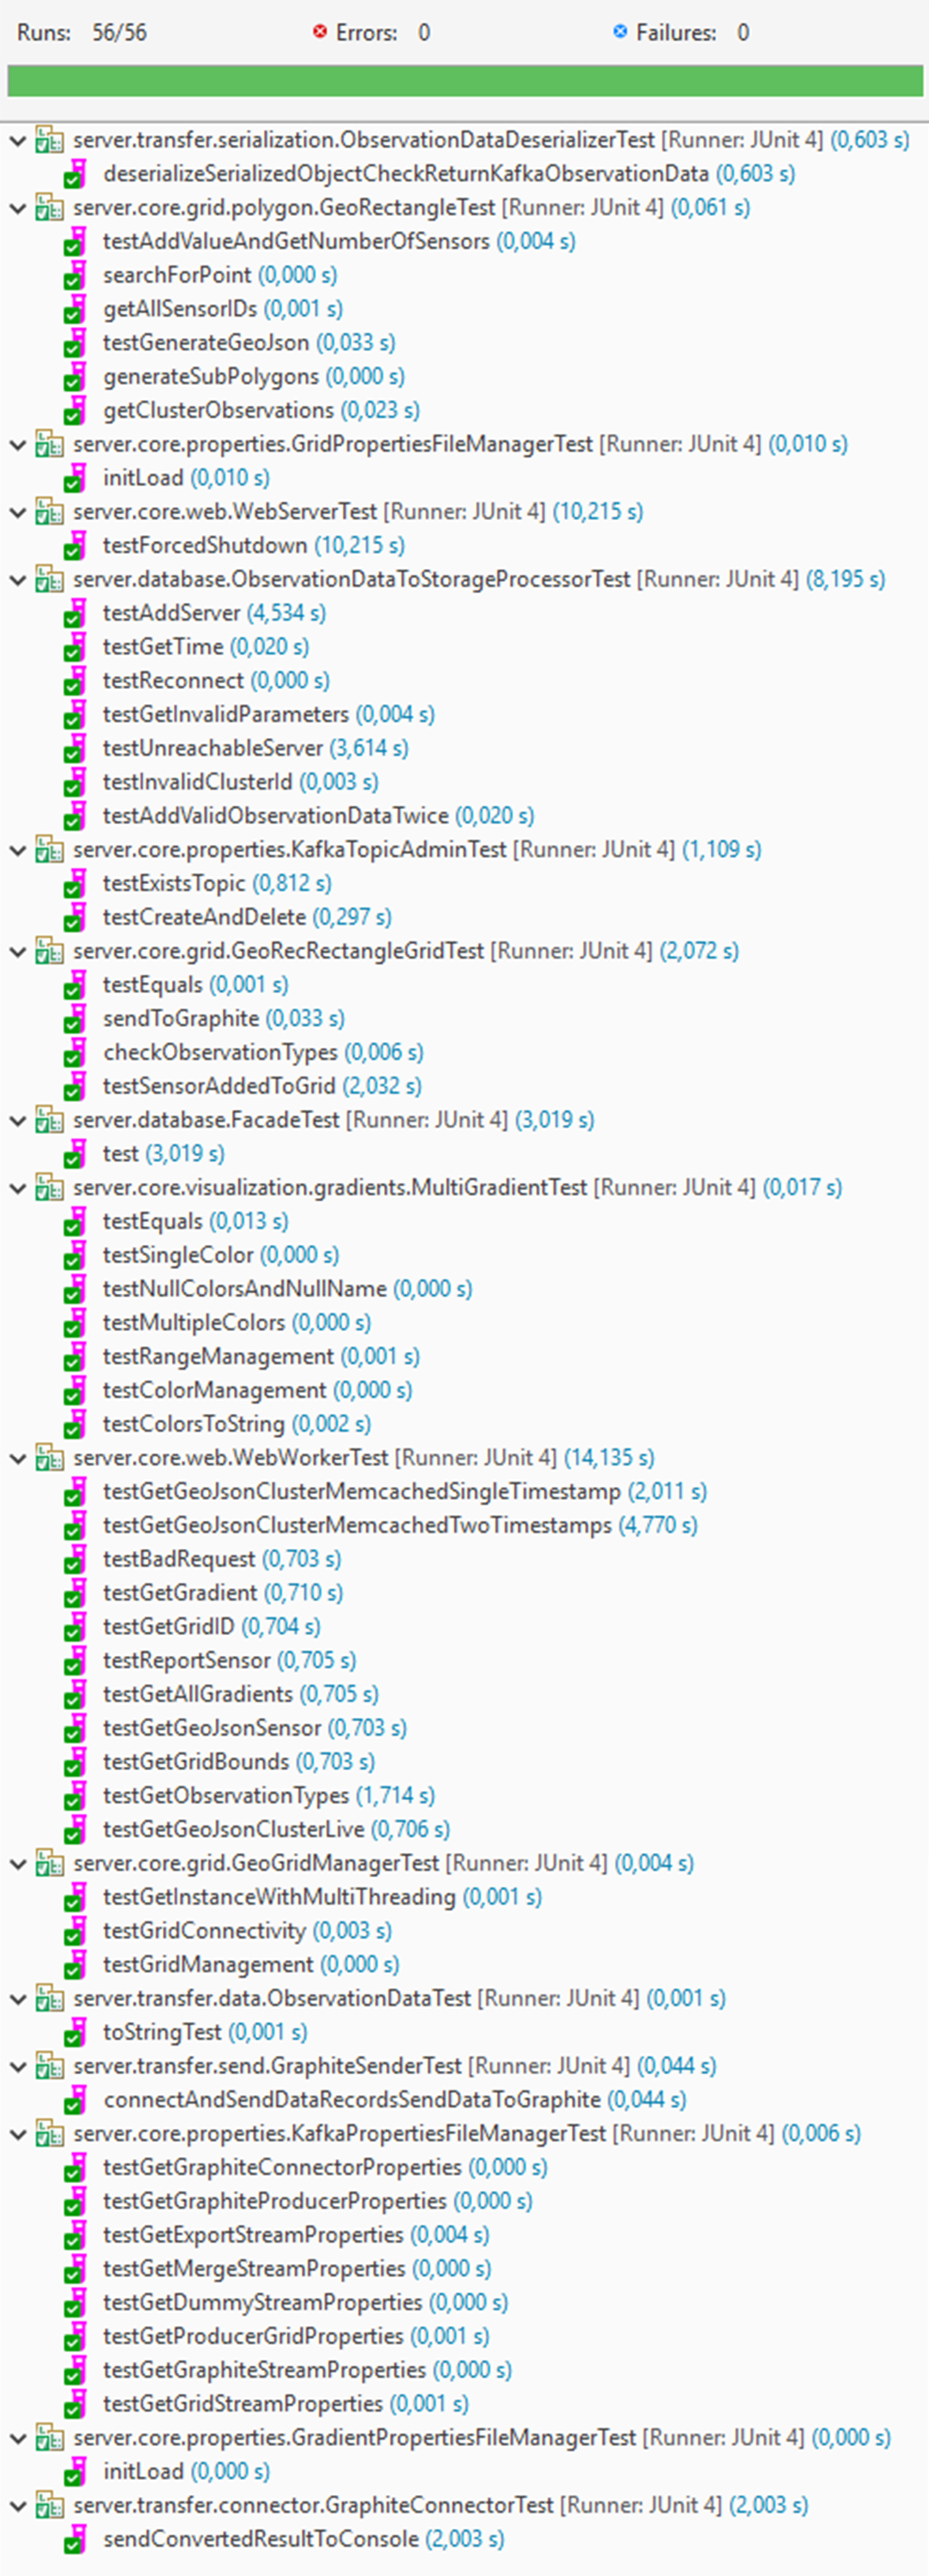
\includegraphics[width=0.6\linewidth]{images/tests}
\end{figure}

\newpage

\begin{figure}
	\centering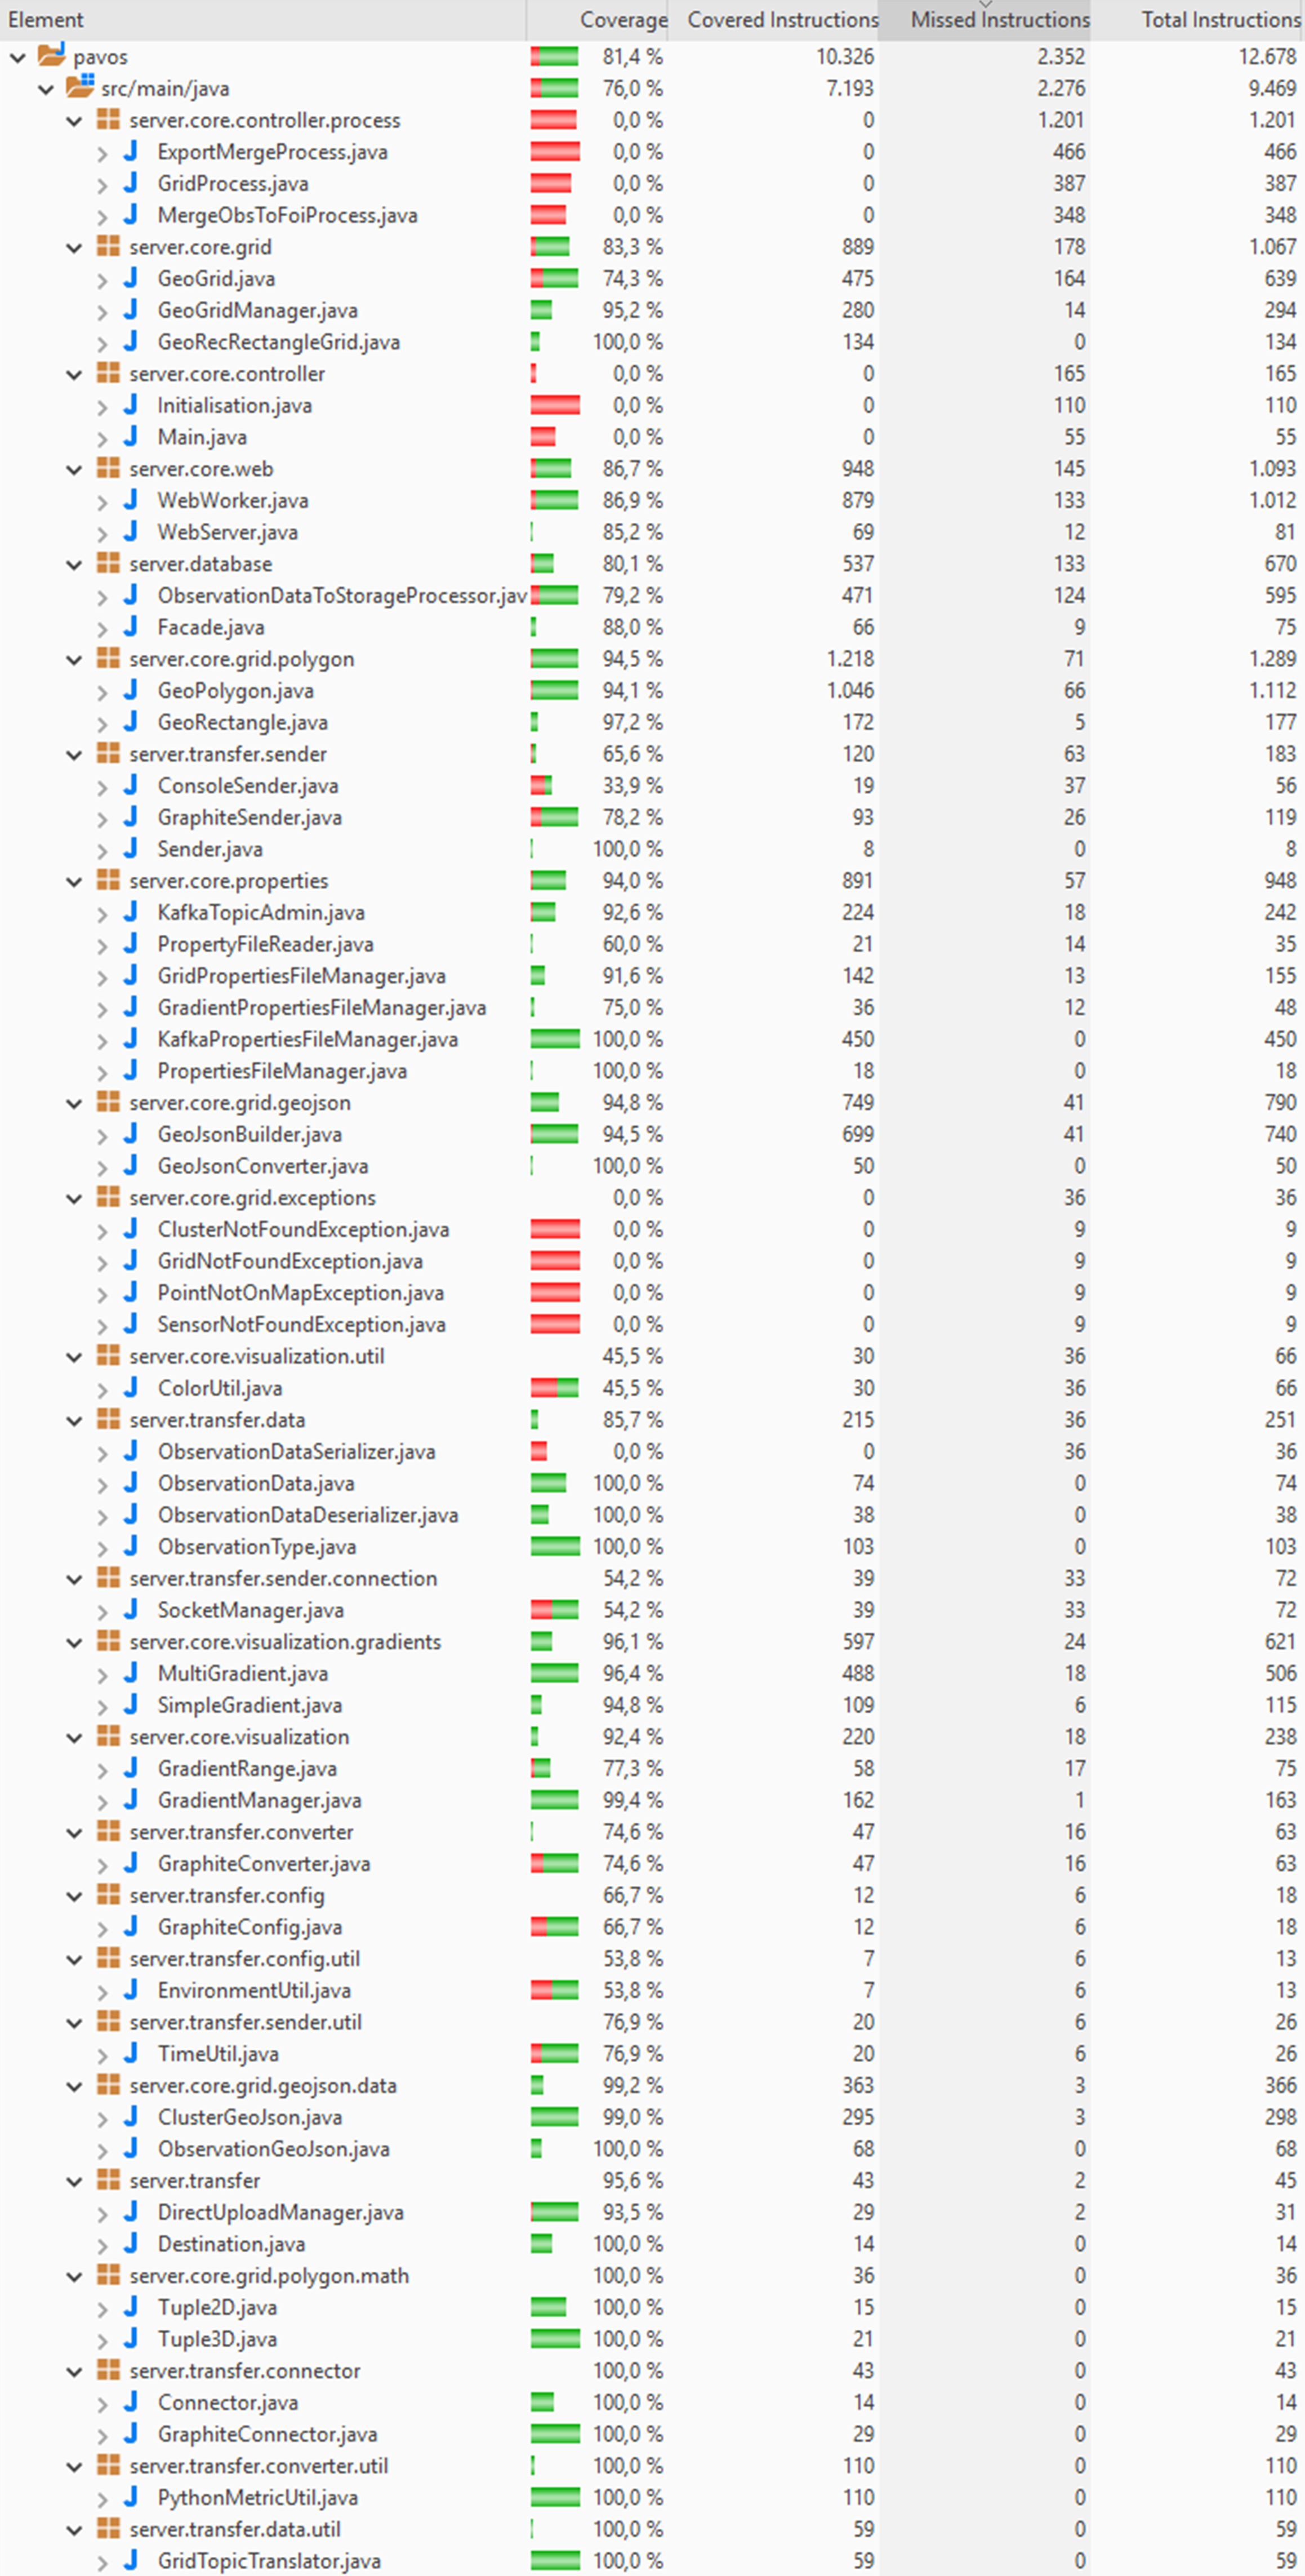
\includegraphics[width=0.84\linewidth]{images/coverage}
\end{figure}

\newpage
\section{Testszenarien}
Hier werden sowohl alte als auch neue Szenarien getestet.
Szenarien, die sich auf die im Pflichtenheft genannten Eintr\"age beziehen werden durch die entsprechende Kennzeichnung (z.B. TI1000) deutlich gemacht. \newline
Die Werte 1000 - 1070 deuten an, dass es sich um Server seitige Tests handelt. \newline
Die Werte 2000 - 2100 deuten an, dass es sich um Client seitige Tests handelt.

\subsection{\"Uberarbeitete Szenarien}
\begin{table}[H]
\centering
\begin{tabular}{|L{1.3cm}|L{7cm}|L{2cm}|}
\hline
Szenario & Grund & Ersetzt durch\\
\hline
TI1000, TI1010, TI1020, TI1030, TI1040, TI1070 & Die Konfigurations-GUI wurde durch Umgebungsvariablen ersetzt und die Prozesse beginnen mit dem Start des Docker-Containers (bzw. mit dem Ausf\"uhren der .jar Datei) automatisch.
\newline
Hieraus ergibt sich, dass die Konfigurations-GUI und deren Einstellungsm\"oglichkeiten \"uberfl\"ussig geworden sind. & - \\ \hline
TI 2000 & Die Übeprüfung der Berechnung des Mittelwerts ist bereits als Unittest im Core abgedeckt. & - \\ \hline
TI1050, TI1060 & Aufgrund oben genannter \"Anderungen und wegen neuen Design-Entscheidungen wurde dieser Teil auf eine vom Kern seperat agierende Komponente verschoben - das Import- / Export- Servlet.
\newline
Mit Hilfe dieses Servlets soll der Benutzer in die Lage versetzt werden, Daten vom Kern zu importieren und Daten zu exportieren. & QS2050, QS1060 \\ \hline
TI2050 & Dieses Szenario wurde mit einem anderen Szenario verschmolzen. & QS2050 \\ \hline
- & Um das Servlet ohne Webinterface testen zu können, wurde ein neues Szenario erstellt. & QS2100 \\ \hline
\end{tabular}
\end{table}

\newpage

\subsection{QS1060 - Import von Daten mit dem Servlet}
\paragraph{Voraussetzungen}
\begin{itemize}
\item FROST-Server
\item Die Adresse des FROST-Servers muss bekannt sein und auf "/v1.0/" enden
\item Importer (pim.jar) muss vorhanden sein
\item Testdateien müssen vorhanden sein (test.csv, multi1test.csv und multi2test.csv)
\end{itemize}
\paragraph{Ablauf}
\begin{enumerate}
\item Starten der pim.jar per Doppelklick oder über die Kommandozeile
\item Folgende UI-Elemente m\"ussen in der ge\"offneten Anwendung zu sehen sein:
\begin{itemize}
\item Zwei Textfelder, das eine mit einem Link, das andere als Text
\item Zwei Kn\"opfe, der eine zum ausw\"ahlen von Dateien, der andere zum Importieren
\item Eine leere Tabelle
\end{itemize}
\item Im oberen Textfeld mit dem Link wird der bekannte Link zum FROST-Server eingefügt werden
\item Im unteren Textfeld wird der Zusatz f\"ur die IoT-IDs eingetragen, der die Daten dieses Imports eindeutig kennzeichnet
\item Als n\"achstes wird der Knopf mit der Aufschrift "Choose Files" gedrückt
\item Es \"offnet sich ein Auswahlfenster
\item Nun werden die Testdaten ausgew\"ahlt
\begin{itemize}
\item Variante 1: nur test.csv
\item Variante 2: multi1test.csv und multi2test.csv
\end{itemize}
\item Alle ausgew\"ahlten Dateien werden in der Tabelle aufgelistet und der Fortschritt betr\"agt 0\%
\item Nun wird der Knopf mit der Aufschrift "Import Files" gedr\"uckt
\item Anschlie\ss end startet der Import und es folgt keine Fehlermeldung
\item Es wird bis zu 5 Minuten gewartet oder bis 100\% Fortschritt erreicht sind
\item Ist der Fortschritt nach dieser Zeit noch nicht bei 100\%, so gilt der Test als nicht bestanden
\item Zur \"Uberpr\"ufung der Daten wird der bekannte Link zum FROST-Server aufgerufen und die Endungen: Sensor, ObservedProperties, Things, FeaturesOfInterest, Datastreams und Observations nach einanander angefügt (den Vorgänger wieder löschend)
\begin{itemize}
\item Variante 1: Es ist genau ein Eintrage für jede Endung vorhanden (ein Eintrag ist hier ein json mit einer IoT-ID)
\item Variante 2: Es sind genau zwei Einträge für jedes vorhanden
\item Die angezeigten IoT-IDs müssen mit dem Inhalt des zweiten angegebenen Texfeldes anfangen
\end{itemize}
\item Zur genauen Prüfung werden die csv-Dateien geöffnet
\item Jede in dem csv enthaltene Information muss auch in Frost vorhanden sein, wobei der erste Eintrag in jeder Zeile gibt immer an, um welchen Typ es sich handelt.
\end{enumerate}
\szenarioGood

\subsection{TI2010 - Darstellung von Clustern ohne Sensoren}
\paragraph{Voraussetzungen}
\begin{itemize}
\item Pavos-Webinterface
\item Verbindung zum Webserver
\end{itemize}
\paragraph{Ablauf}
\begin{enumerate}
\item Das Webinterface wird im Browser geöffnet
\item Das Webinterface wird in den manuellen Historischen Modus überführt:
\begin{enumerate}
\item Falls nicht bereits im Historischen Modus, den Knopf mit dem Refresh Symbol rechts vom "Settings" Knopf anklicken und das Webinterface ist nun im Historischen Modus
\item Falls nicht bereits im manuellen Modus, den Knopf mit der Aufschrift "Settings" anklicken
\item Es öffnet sich ein Overlay mit dem Titel "Settings"
\item Unter der Kategorie "Automatic/Manual Refresh'' den Radiobutton "Manual'' auswählen
\item Es wird auf den Knopf mit der Aufschrift "Apply" geklickt und das Webinterface ist nun im manuellen Modus
\end{enumerate}
\item Den Knopf mit der Aufschrift "Settings" wird geklickt
\item Es öffnet sich ein Overlay mit dem Titel "Settings"
\item Im Feld "From" wird ein Datum ausgewählt an welchem keine Sensordaten zur Verfügung stehen
\item Im Feld "To" wird ein späteres Datum eingetragen
\item Es wird der Knopf "Apply" geklickt und das Overlay schließt sich
\item Es wird der Refresh Knopf links neben dem "Settings" Knopf gedrückt
\item Das Grid auf der Karte ist nun leer und nur die Karte an sich wird angezeigt
\end{enumerate}
\szenarioOk

\subsection{TI2020 - Darstellung der Tabellarischen Ansicht}
\paragraph{Voraussetzungen}
\begin{itemize}
\item Pavos-Webinterface
\item Verbindung zum Webserver
\end{itemize}
\paragraph{Ablauf}
\begin{enumerate}
\item Das Webinterface wird im Browser geöffnet
\item Das Webinterface wird in den automatisierten Live-Modus überführt:
\begin{enumerate}
\item Falls nicht bereits im Live-Modus, den Knopf mit dem Sanduhr Symbol rechts vom "Settings" Knopf anklicken und das Webinterface ist nun im Live-Modus
\item Falls nicht bereits im automatisierten Modus, den Knopf mit der Aufschrift "Settings" anklicken
\item Es öffnet sich ein Overlay mit dem Titel "Settings"
\item Unter der Kategorie "Automatic/Manual Refresh'' den Radiobutton "Automatic'' auswählen
\item Es wird auf den Knopf mit der Aufschrift "Apply" geklickt und das Webinterface ist nun im automatisierten Modus
\end{enumerate}
\item Es wird der Start Knopf links neben dem "Settings" Knopf gedrückt
\item Auf der Karte wird bis zum größten Grid Level gezoomt:
\begin{enumerate}
\item Es wird so lange gezoomt bis das Grid nicht mehr kleinteiliger wird
\end{enumerate}
\item Es wird ein Cluster selektiert
\item In der Tabelle werden die Bezeichner aller Sensoren dargestellt, die sich im selektierten Cluster befinden
\end{enumerate}
\szenarioOk

\subsection{TI2030 - Benutzen mehrerer Webinterface-Instanzen}
\paragraph{Voraussetzungen}
\begin{itemize}
\item Pavos-Webinterface
\item Verbindung zum Webserver
\end{itemize}
\paragraph{Ablauf}
\begin{enumerate}
\item Das Webinterface wird in zwei verschiedenen Browser Fenstern mit derselben Kartenposition und demselben Kartenzoom geöffnet, sowie auf dem Bildschirm nebeneinander positioniert
\item Die Webinterface Instanzen werden beide in den manuellen Live-Modus überführt:
\begin{enumerate}
\item Falls nicht bereits im Live-Modus, den Knopf mit dem Sanduhr Symbol rechts vom "Settings" Knopf anklicken und das Webinterface ist nun im Live-Modus
\item Falls nicht bereits im manuellen Modus, den Knopf mit der Aufschrift "Settings" anklicken
\item Es öffnet sich ein Overlay mit dem Titel "Settings"
\item Unter der Kategorie "Automatic/Manual Refresh'' den Radiobutton "Manual'' auswählen
\item Es wird auf den Knopf mit der Aufschrift "Apply" geklickt und das Webinterface ist nun im manuellen Modus
\end{enumerate} 
\item Es wird bei beiden Webinterface Instanzen auf den Refresh Knopf  links neben dem "Settings" Knopf gedrückt und die momentane Live-Ansicht angefordert
\item Auf der Karte wird bei beiden Webinterface Instanzen das gleiche Raster mit denselben Farben dargestellt und der Inhalt der Tabelle ist gleich
\end{enumerate}
\szenarioGood

\subsection{TI2040 - Auswahl eines Sensortyps}
\paragraph{Voraussetzungen}
\begin{itemize}
\item Pavos-Webinterface
\item Verbindung zum Webserver
\end{itemize}
\paragraph{Ablauf}
\begin{enumerate}
\item Das Webinterface wird im Browser geöffnet
\item Der Knopf mit der Aufschrift "Sensortype" wird  geklickt
\item Es öffnet sich ein Overlay mit dem Titel "Sensortype"
\item Unter der Kategorie "Choose Sensortype" wird ein anderer Sensortyp Radiobutton ausgewählt
\item Es wird auf den Knopf mit der Aufschrift "Apply" geklickt und der Sensortyp wurde geändert
\end{enumerate}
\szenarioGood

\subsection{QS2050 - Export von Daten mit dem Servlet}
\paragraph{Voraussetzungen}
\begin{itemize}
\item FROST-Server
\item Kafka-System
\item Pavos-Bridge zwischen FROST und Kafka
\item Pavos-Core
\item Export-Docker
\item Pavos-Webinterface
\item Ein abgeschlossener Import-Test auf diesem System
\item Keine weiteren eingespeisten Daten auf dem System
\end{itemize}
\paragraph{Ablauf}
\begin{enumerate}
\item Das Webinterface wird im Browser geöffnet
\item Auf der Karte wird ein Cluster ausgewählt, das Deutschland enthält
\item Der Knopf mit der Aufschrift "Export"
\item Es öffnet sich ein Overlay mit dem Titel Export in das folgendes eingetragen wird:
\begin{itemize}
\item Im Feld "From" wird das Datum von vor einem Monat eingetragen
\item Im Feld "To" wird das aktuelle Datum eingetragen
\item Im Menüpunkt  "Choose Clusters" wird "All Selected" ausgewählt
\item In der Kategorie "Choose Sensortype" wird "temperature\textunderscore celsius" ausgewählt
\item In der Kategorie "Choose Exportformat" wird "CSV" ausgewählt
\item Es wird auf den Knopf mit der Aufschrift "Apply" geklickt
\item Die Exportierten Daten werden nach spätestens 5 Minuten heruntergeladen
\end{itemize}
\end{enumerate}
\szenarioGood

\subsection{TI2060 - Wiederholungen anzeigen}
\paragraph{Voraussetzungen}
\begin{itemize}
\item Pavos-Webinterface
\item Verbindung zum Webserver
\end{itemize}
\paragraph{Ablauf}
\begin{enumerate}
\item Das Webinterface wird im Browser geöffnet
\item Das Webinterface wird in den automatisierten Historischen Modus überführt:
\begin{enumerate}
\item Falls nicht bereits im Historischen Modus, den Knopf mit dem Refresh Symbol rechts vom "Settings" Knopf anklicken und das Webinterface ist nun im Historischen Modus
\item Falls nicht bereits im automatisierten Modus, den Knopf mit der Aufschrift "Settings" anklicken
\item Es öffnet sich ein Overlay mit dem Titel "Settings"
\item Unter der Kategorie "Automatic/Manual Refresh'' den Radiobutton "Automatic'' auswählen
\item Es wird auf den Knopf mit der Aufschrift "Apply" geklickt und das Webinterface ist nun im automatisierten Modus
\end{enumerate}
\item Der Knopf mit der Aufschrift "Settings" wird geklickt
\item Es öffnet sich ein Overlay mit dem Titel "Settings"
\item Im Feld "From" wird das Datum von vor einem Monat eingetragen
\item Im Feld "To" wird das Datum von gestern eingetragen
\item Es wird der Knopf "Apply" geklickt und das Overlay schließt sich
\item Es wird der Start Knopf links neben dem "Settings" Knopf gedrückt
\item Das Grid auf der Karte visualisiert nun die Iteration über eine festgelegte Anzahl an Zeitpunkten zwischen dem zuvor festgelegten From und To Zeitpunkten
\end{enumerate}
\szenarioGood

\subsection{TI2070 - Echtzeitdarstellung}
\paragraph{Voraussetzungen}
\begin{itemize}
\item Pavos-Webinterface
\item Verbindung zum Webserver
\end{itemize}
\paragraph{Ablauf}
\begin{enumerate}
\item Das Webinterface wird im Browser geöffnet
\item Das Webinterface wird in den automatisierten Live-Modus überführt:
\begin{enumerate}
\item Falls nicht bereits im Live-Modus, den Knopf mit dem Sanduhr Symbol rechts vom "Settings" Knopf anklicken und das Webinterface ist nun im Live-Modus
\item Falls nicht bereits im automatisierten Modus, den Knopf mit der Aufschrift "Settings" anklicken
\item Es öffnet sich ein Overlay mit dem Titel "Settings"
\item Unter der Kategorie "Automatic/Manual Refresh'' den Radiobutton "Automatic'' auswählen
\item Es wird auf den Knopf mit der Aufschrift "Apply" geklickt und das Webinterface ist nun im automatisierten Modus
\end{enumerate}
\item Es wird der Start Knopf links neben dem "Settings" Knopf gedrückt
\item Das Grid auf der Karte wird nun regelmäßig in festen Intervallen mit Live-Daten aktualisiert
\end{enumerate}
\szenarioGood

\subsection{TI2080 - Detailansicht eines Sensors}
\paragraph{Voraussetzungen}
\begin{itemize}
\item Pavos-Webinterface
\item Verbindung zum Webserver
\end{itemize}
\paragraph{Ablauf}
\begin{enumerate}
\item Das Webinterface wird im Browser geöffnet
\item Das Webinterface wird in den automatisierten Live-Modus überführt:
\begin{enumerate}
\item Falls nicht bereits im Live-Modus, den Knopf mit dem Sanduhr Symbol rechts vom "Settings" Knopf anklicken und das Webinterface ist nun im Live-Modus
\item Falls nicht bereits im automatisierten Modus, den Knopf mit der Aufschrift "Settings" anklicken
\item Es öffnet sich ein Overlay mit dem Titel "Settings"
\item Unter der Kategorie "Automatic/Manual Refresh'' den Radiobutton "Automatic'' auswählen
\item Es wird auf den Knopf mit der Aufschrift "Apply" geklickt und das Webinterface ist nun im automatisierten Modus
\end{enumerate} 
\item Es wird der Start Knopf links neben dem "Settings" Knopf gedrückt
\item Auf der Karte wird bis zum größten Grid Level gezoomt:
\begin{enumerate}
\item Es wird so lange gezoomt bis das Grid nicht mehr kleinteiliger wird
\end{enumerate}
\item Es wird ein Cluster selektiert
\item In der Tabelle werden die Bezeichner aller Sensoren dargestellt, die sich im selektierten Cluster befinden
\item Klicke einen Eintrag in der Tabelle
\item Es öffnet sich ein Overlay mit dem Sensor Bezeichner als Titel
\item Es wird der Knopf "Show" geklickt und das Overlay schließt sich
\item Der Verlauf des Sensors wird im Grafen angezeigt
\end{enumerate}
\szenarioGood

\subsection{TI2090 - Melden eines Sensors}
\paragraph{Voraussetzungen}
\begin{itemize}
\item Pavos-Webinterface
\item Verbindung zum Webserver

% Hier muss noch rein was man braucht um in den Logs nachzusehen dass ein Sensor reported wurde
\item =========================================================

\end{itemize}
\paragraph{Ablauf}
\begin{enumerate}
\item Das Webinterface wird im Browser geöffnet
\item Das Webinterface wird in den automatisierten Live-Modus überführt:
\begin{enumerate}
\item Falls nicht bereits im Live-Modus, den Knopf mit dem Sanduhr Symbol rechts vom "Settings" Knopf anklicken und das Webinterface ist nun im Live-Modus
\item Falls nicht bereits im automatisierten Modus, den Knopf mit der Aufschrift "Settings" anklicken
\item Es öffnet sich ein Overlay mit dem Titel "Settings"
\item Unter der Kategorie "Automatic/Manual Refresh'' den Radiobutton "Automatic'' auswählen
\item Es wird auf den Knopf mit der Aufschrift "Apply" geklickt und das Webinterface ist nun im automatisierten Modus
\end{enumerate} 
\item Es wird der Start Knopf links neben dem "Settings" Knopf gedrückt
\item Auf der Karte wird bis zum größten Grid Level gezoomt:
\begin{enumerate}
\item Es wird so lange gezoomt bis das Grid nicht mehr kleinteiliger wird
\end{enumerate}
\item Es wird ein Cluster selektiert
\item In der Tabelle werden die Bezeichner aller Sensoren dargestellt, die sich im selektierten Cluster befinden
\item Klicke einen Eintrag in der Tabelle
\item Es öffnet sich ein Overlay mit dem Sensor Bezeichner als Titel
\item Unter der Kategorie "Report Reason" wird "Report Test" im Textfeld eingetragen
\item Der Knopf "Report" wird geklickt

\item ========================================================

% Hier muss rein was man tut um nachzugucken ob der Report erfolgreich war

\end{enumerate}
\szenarioOk

\subsection{QS2100 - Direktes Ansprechen des Servlets}
\paragraph{Voraussetzungen}
\begin{itemize}
\item FROST-Server
\item Kafka
\item Pavos-Bridge zwischen FROST und Kafka
\item Pavos-Core mit Daten gefüttert
\item Export-Docker
\item Der Link zum Export-Servlet muss bekannt sein (endet auf "/edms/get?" vor der Angabe von Parametern). Dieser Link wird hier Beispielhaft als SERVLET? gekürzt.
\end{itemize}
\paragraph{Ablauf}
\subparagraph{Test 1 - Erlaubte Dateiendungen abfragen}
\begin{enumerate}
\item Der Link "SERVLET?requestType=getExtensions" wird im Browser aufgerufen
\item Die Webseite enthält nur Text
\item Dieser Text ist eine mit Komma separierte Liste aller erlaubter Dateiendungen für den Export der Daten
\item Die Liste enthält mindestens einen Eintrag (normalerweise csv)
\end{enumerate}
\subparagraph{Test 2 - Nicht vorhandene Datei}
\begin{enumerate}
\item Der Link "SERVLET?requestType=getStatus\& downloadID=test" wird im Browser aufgerufen
\item Die Webseite enthält nur Text
\item Der Text ist "noID"
\item Der Link "SERVLET?requestType=tryDownload\& downloadID=test" wird im Browser aufgerufen
\item Es wird eine Http-Fehlermeldung zurückgegeben
\end{enumerate}
\subparagraph{Test 3 - Datei exportieren}
Hier muss bekannt sein, welche Messgrößen (z.B. "temperature\textunderscore celsius"), welche erlaubten Export-Dateiendungen und welche Cluster (ID muss bekannt sein) existieren.
\begin{enumerate}
\item Es wird aus den bekannten Messgrößen, Export-Dateiendungen und Clustern jeweils eins ausgewählt
\item Der Link "SERVLET?requestType=newExport\& downloadID=test\& extension=FORMAT\& timeFrame= DATES:ssZ\& observedProperties=\newline OBSERVEDPROPERTIES\& clusters=CLUSTER"
\par
Wobei FORMAT gleich der ausgewählten Export-Dateiendung entspricht. DATES, wird durch einen Datums-Bereich der zu importierenden Sensor-Werte im Format YYYY-MM-DDThh:mm:ssZ mit Komma getrennt (und mit maximal zwei Daten) ersetzt. OBSERVEDPROPERTIES entspricht der ausgesuchten Messgröße und CLUSTER dem ausgesuchten Cluster.
\item Es wird "started" als Text zurückgegeben
\item Der Link wird ein zweites mal aufgerufen
\item Es wird "duplicate" als Text zurückgegeben
\item Der Link "Servlet?requestType=getStatus\& downloadID=test" wird im Browser aufgerufen
\item Die Webseite enthält nur Text
\item Dieser Text ist entweder "false" oder "true"
\item Wird "false" zurückgegeben, muss solange gewartet oder neu geladen werden, bis "true" zurückgegeben wird. 
\newline
Die Wartezeit skaliert mit der Größe der Anfrage und sollte bei kleinen Größen 10 Minuten betragen.
\item Sobald "true" zurückgegeben wird, wird automatisch eine Datei namens "test.zip" heruntergeladen, die die exportierten Daten enthält.
\end{enumerate}
\szenarioGood